\documentclass[12pt, twoside]{article}
\usepackage[letterpaper, margin=1in, head=30pt, headsep=0.1in]{geometry}
\usepackage[english]{babel}
\usepackage[utf8]{inputenc}
\usepackage{amsmath}
\usepackage{amsfonts}
\usepackage{amssymb}
\usepackage{tikz}
\usepackage{yhmath} %arcs using \wideparen{}
\usetikzlibrary{quotes, angles}

\usepackage{graphicx}
\usepackage{enumitem}
\usepackage{multicol}

%\usepackage{pgfplots}
%\pgfplotsset{width=10cm,compat=1.9}
%\usepgfplotslibrary{statistics}
%\usepackage{pgfplotstable}
%\usepackage{tkz-fct}
%\usepackage{venndiagram}

\usepackage{fancyhdr}
\pagestyle{fancy}
\fancyhf{}
\renewcommand{\headrulewidth}{0pt} % disable the underline of the header
\raggedbottom
\newif\ifmeta
\metatrue %print standards and topics tags

\title{High School Geometry problem sets}
\author{Chris Huson}
\date{April 2021}

%\fancyhead[RE]{\thepage}
%\fancyhead[RO]{\thepage \\ Name: \hspace{3cm}}
%\fancyhead[L]{BECA / Dr. Huson / 10th Grade Geometry\\* 7 June 2019}
%
%\begin{document}
%\subsubsection*{13.7 Homework: Cross sections, distance applications}
%\fancyhead[L]{BECA / Dr. Huson / Geometry 03-Volume+angle-bisectors\\* pset ID: 34}

\begin{document}

\subsubsection*{7.9 Angle review}
\begin{enumerate}
\item The size of an angle is its ``measure,'' which can be from $0^\circ$ to $360^\circ$
\begin{enumerate}
  \item What is the degree measure of the angle, $m\angle PQR$? \\[0.25cm]
  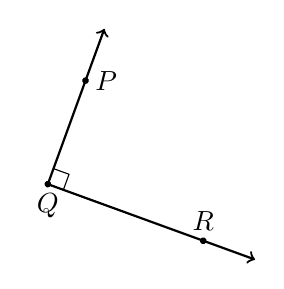
\begin{tikzpicture}[scale=0.7, rotate=-20]
    \draw [<->, thick] (4,0)--(0,0)--(0,3);
    \draw (0,0)++(0.3,0)--++(0,0.3)--+(-0.3,0);
    %\draw [fill] (-1,2.5) circle [radius=0.05] node[left ]{$B$};
    \draw [fill] (0,0) circle [radius=0.05] node[below]{$Q$};
    \draw [fill] (0,2) circle [radius=0.05] node[right]{$P$};
    \draw [fill] (3,0) circle [radius=0.05] node[above]{$R$};
  \end{tikzpicture}
  \item What is the degree measure made by these two opposite rays, $\overrightarrow{BA}$ and $\overrightarrow{BC}$?
  \begin{flushright}
    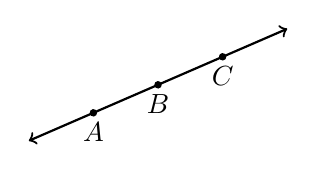
\begin{tikzpicture}[scale=.8, rotate=50]
      \draw  [<->, thick] (0,2)--(4,0);
      \draw [fill] (1,1.5) circle [radius=0.05] node[below]{$A$};
      \draw [fill] (2,1) circle [radius=0.05] node[below]{$B$};
      \draw [fill] (3,0.5) circle [radius=0.05] node[below]{$C$};
    \end{tikzpicture}
  \end{flushright}
    \item The given angle $\angle UVW$ is which of the following: acute, obtuse, or right?
    \begin{center}
      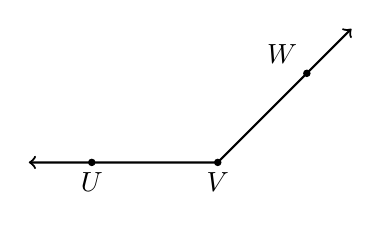
\begin{tikzpicture}[scale=.8]
        \draw  [<->, thick] (-3,0)--(0,0)--(45:3);
        \draw [fill] (-2,0) circle [radius=0.05] node[below]{$U$};
        \draw [fill] (0,0) circle [radius=0.05] node[below]{$V$};
        \draw [fill] (45:2) circle [radius=0.05] node[above left]{$W$};
      \end{tikzpicture}
    \end{center}
  \end{enumerate}

\newpage
\item As shown below, two lines intersect making four angles: $\angle 1$, $\angle 2$, $\angle 3$, and $\angle 4$.

  \begin{multicols}{2}
    Given $m\angle 2 = 110^\circ$.  
    \begin{enumerate}
      \item Find $m\angle 3$ \vspace{2cm}
      \item Find $m\angle 4$ \vspace{2cm}
    \end{enumerate}
    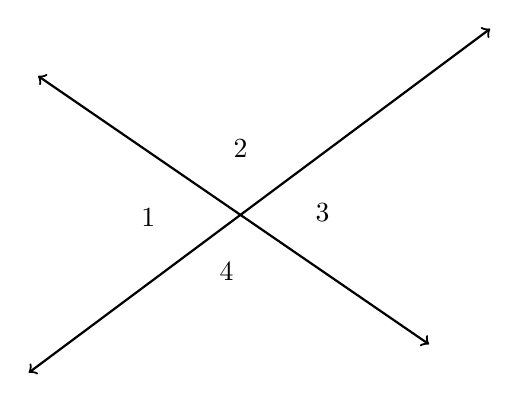
\begin{tikzpicture}[scale=0.7, rotate=20]
    \draw [<->, thick] (0,-1.5)--(10,1.5);
    \draw [<->, thick] (2,3.5)--(7,-3.5);
    \node at (3,.4){1};
    \node at (6,-.6){3};
    \node at (5,1){2};
    \node at (4,-1){4};
  \end{tikzpicture}
  \end{multicols}

\newpage
\item Apply the Angle Addition postulate. Write and equation to support your work.
  \begin{multicols}{2}
    Given $m\angle CBD = 30^\circ$, $m\angle ABC = 90^\circ$. \\[0.5cm]
    Find $m \angle ABD$. \\
    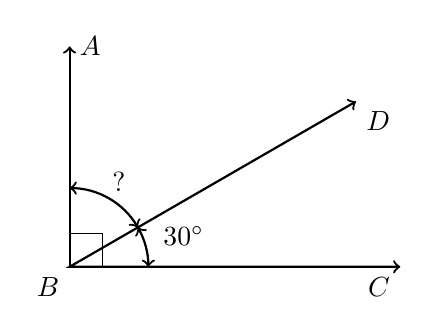
\begin{tikzpicture}[scale=1.4]
      \draw [<->, thick]
        (0:3) coordinate (a) node[below left] {$C$}
        -- (0,0) coordinate (b) node[below left] {$B$}
        -- (30:3) coordinate (c) node[below right] {$D$}
        pic["$30^\circ$", <->, draw=black, angle eccentricity=1.5, angle radius=1cm]
        {angle=a--b--c};
        \draw [<-, thick]
        (90:2) coordinate (d) node[right] {$A$}
        -- (0,0) coordinate (e)
        pic["$?$", <->, draw=black, angle eccentricity=1.25, angle radius=1cm]
        {angle=c--e--d};
      \draw (0,0)++(0.3,0)--++(0,0.3)--+(-0.3,0);
    \end{tikzpicture}
  \end{multicols}

\newpage
\item Given $\overrightarrow{BD} \perp \overleftrightarrow{ABC}$, $m\angle DBE = 2x$, and $m\angle EBC = x - 15^\circ$, as shown below. \\[0.5cm] 
Write an equation and solve for $x$.
  \begin{flushright}
    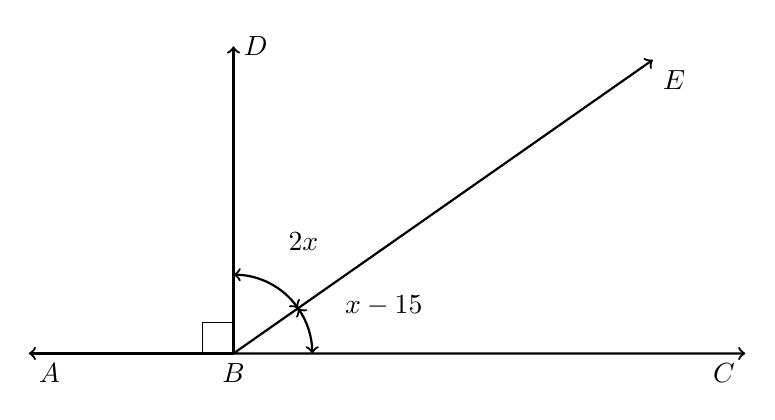
\begin{tikzpicture}[scale=1.3]
      \draw [<->, thick]
        (0:5) coordinate (a) node[below left] {$C$}
        -- (0,0) coordinate (b) node[below] {$B$}
        -- (35:5) coordinate (c) node[below right] {$E$}
        pic["$x-15$", <->, draw=black, angle eccentricity=2, angle radius=1cm]
        {angle=a--b--c};
        \draw [<-, thick]
        (90:3) coordinate (d) node[right] {$D$}
        -- (0,0) coordinate (e)
        pic["\hspace{0.3cm}$2x$", <->, draw=black, angle eccentricity=1.6, angle radius=1cm]
        {angle=c--e--d};
        \draw [->, thick] (0,0)--(-180:2) node[below right]{$A$};
        \draw (0,0)++(-0.3,0)--++(0,0.3)--+(0.3,0);
    \end{tikzpicture}
  \end{flushright}
  %https://graspablemath.com/canvas?load=_bb77d88dbfd6a8ba
  
\newpage
\item An equilateral triangle is inscribed in a circle with a radius $r=9$. Find each:
  \begin{multicols}{2}
  \raggedcolumns
  \begin{enumerate}[itemsep=1.1cm]
    \item $m \angle AOB$
    \item The circle circumference. ($C=2\pi r$)
    \item The length of the arc $\wideparen{AB}$
    \item The circle's area. ($A=\pi r^2$)
    \item The sector area (in gray)
  \end{enumerate}
  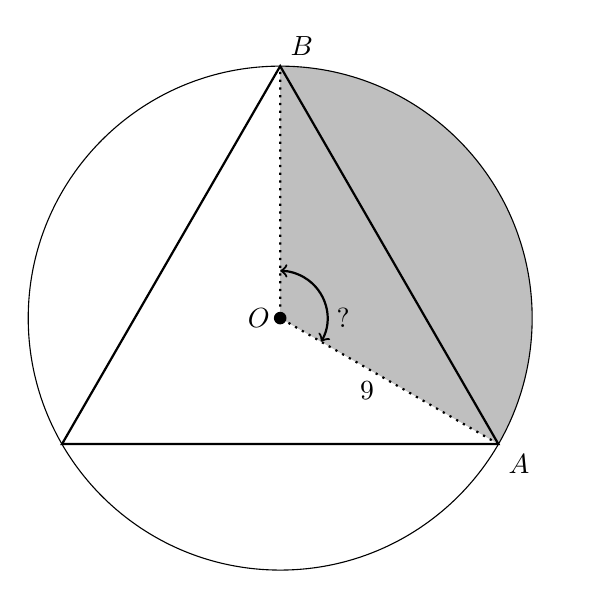
\begin{tikzpicture}[scale=0.8]
    \fill [lightgray]
    (0,0)--(-30:4) arc (-30:90:4)--(0,0);
    \draw (0,0) circle[radius=4];
    \draw [thick, <->] (-30:0.75) arc (-30:90:0.75);
    \draw [thick, dotted]
    (-30:4) node[below right] {$A$}--
    (0,0) node[left] {$O$}--
    (90:4) node[above right] {$B$};
    \draw [thick]
    (-30:4) -- (90:4)-- (210:4)--cycle;
    \fill (0,0) circle[radius=.1];
    \node at (0:1) {$?$};
    \node at (-40:1.8) {$9$};
  \end{tikzpicture}
  \end{multicols}
  
\newpage
\item Given $m\angle B=40^\circ$ and $m\angle ECA=105^\circ$. 
\begin{multicols}{2}
  \raggedcolumns
  \begin{enumerate}[itemsep=1.1cm]
    \item What is the sum of the measures of a triangle's angles? (for example, $\angle BCE$, $\angle B$, and $\angle E$)
    \item Find $m\angle BCE$.
    \item Find $m\angle E$.
  \end{enumerate}
  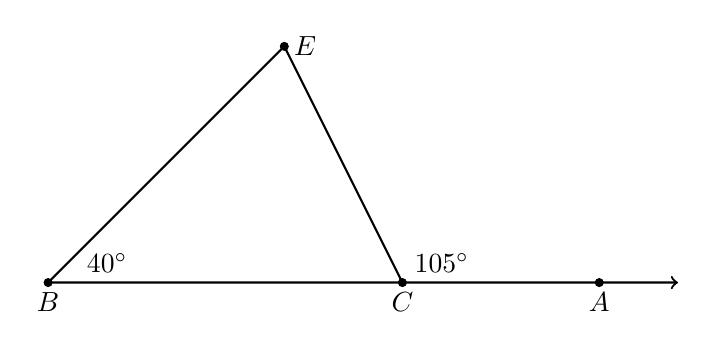
\begin{tikzpicture}
    %\draw [->, thick] (0,0)--(5,5);
    \draw [<-, thick] (8,0)--(0,0)--(3,3)--(4.5,0);
    \draw [fill] (0,0) circle [radius=0.05] node[below]{$B$};
    \draw [fill] (4.5,0) circle [radius=0.05] node[below]{$C$};
    \draw [fill] (3,3) circle [radius=0.05] node[right]{$E$};
    \draw [fill] (7,0) circle [radius=0.05] node[below]{$A$};
    \node at (0.75, 0.25) {$40^\circ$};
    \node at (5, 0.25) {$105^\circ$};
  \end{tikzpicture}
\end{multicols}

\newpage
\item Given circle $O$ with $m \wideparen{HT}=58^\circ$.
  \begin{multicols}{2}
    \raggedcolumns
    \begin{enumerate}
      \item Write down the $m\angle HOT$. \vspace{1.7cm}
      \item Find the $m\angle HAT$. \vspace{2cm}
    \end{enumerate}
      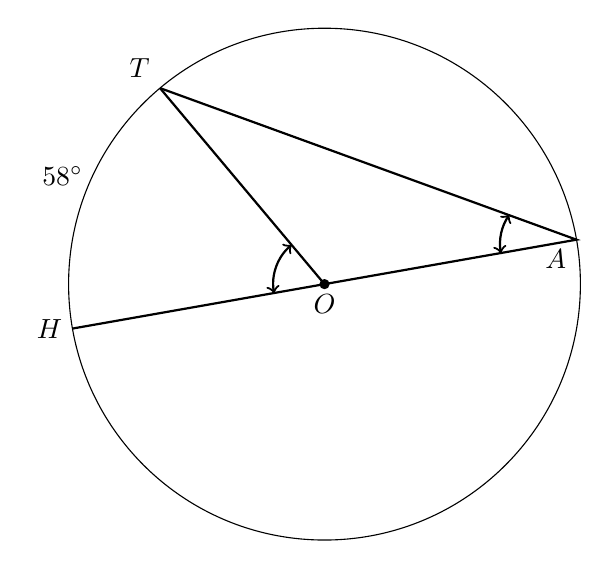
\begin{tikzpicture}[scale=.65]
        \draw (0,0) circle[radius=5];
        \fill (0,0) circle[radius=.1];
        \draw [thick]
        (190:5) node[left] {$H$}--
        (0,0) node[below] {$O$}--
        (130:5) node[above left] {$T$};
        \draw [thick] (0,0)--(10:5) node[below left] {$A$}--(130:5);
        \draw (155:5) node[left]{$58^\circ$};
        \draw [thick, <->] (130:1) arc (130:190:1);
        \draw [thick, <->] (10:3.5) arc (190:145:1);
      \end{tikzpicture}
  \end{multicols}

\newpage
\item Given circle $O$, diameters $\overline {AC}$ and $\overline {BD}$, and arc measure $m \wideparen{BC}= 45^\circ$.
    \begin{multicols}{2}
    \raggedcolumns
    \begin{enumerate}[itemsep=0.5cm]
      \item How are $\angle {AOD}$ and $\angle {BOC}$ related?
      \begin{itemize}
        \item Vertical angles
        \item Opposite angles
        \item Complementary angles
        \item Supplementary angles
        \item Linear pair
      \end{itemize}
      \item Write down $m \angle {AOD}$
      \item Write down $m \wideparen{AD}$.
      \item Find $m \wideparen{AB}$
    \end{enumerate}
    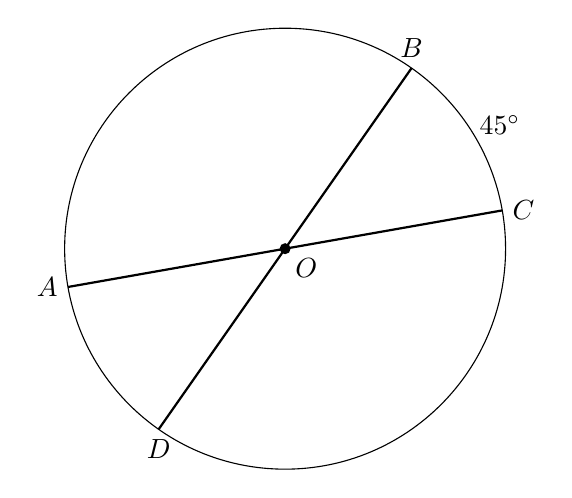
\begin{tikzpicture}[scale=0.7]
      \draw (0,0) circle[radius=4];
      \draw [thick]
      (190:4) node[left] {$A$}--
      (0,0) node[below right] {$O$}--
      (10:4) node[right] {$C$};
      \draw [thick]
      (235:4) node[below] {$D$} -- (55:4) node[above] {$B$};
      \fill (0,0) circle[radius=.1];
      \node at (30:4.5) {$45^\circ$};
    \end{tikzpicture}
    \end{multicols}
  
\newpage
\item Given circle $P$ with $m \wideparen{AB}=70^\circ$.
  \begin{multicols}{2}
    \raggedcolumns
    \begin{enumerate}
      \item Write down the $m\angle APB$. \vspace{1.7cm}
      \item Find the $m\angle AQB$. \vspace{2cm}
    \end{enumerate}
      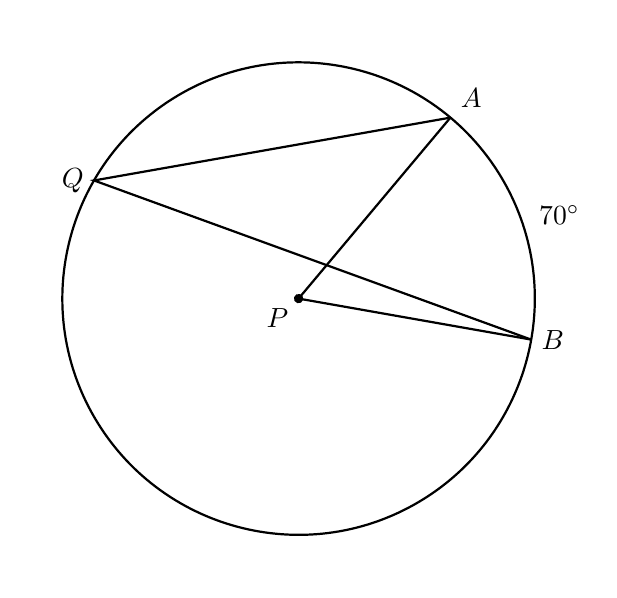
\begin{tikzpicture}[scale=.6, rotate=-60]
        \draw [thick] (0,0) circle[radius=5];
        \fill (0,0) circle[radius=.1];
        \draw [thick]
        (50:5) node[right] {$B$}--
        (0,0) node[below left] {$P$}--
        (110:5) node[above right] {$A$};
        \draw [thick] (50:5)--(210:5) node[left] {$Q$}--(110:5);
        \draw (80:5.2) node[right]{$70^\circ$};
      \end{tikzpicture}
  \end{multicols}

\newpage
\item Ray $\overrightarrow{BF}$ is the angle bisector of $\angle ABC$. Given that the angle measures are $m\angle ABF = 7x-14$ and $m\angle CBF = 5x+10$. \\[0.5cm] 
  Find $x$ and hence, $m\angle ABC$. \vspace{0.5cm}
    \begin{flushright}
      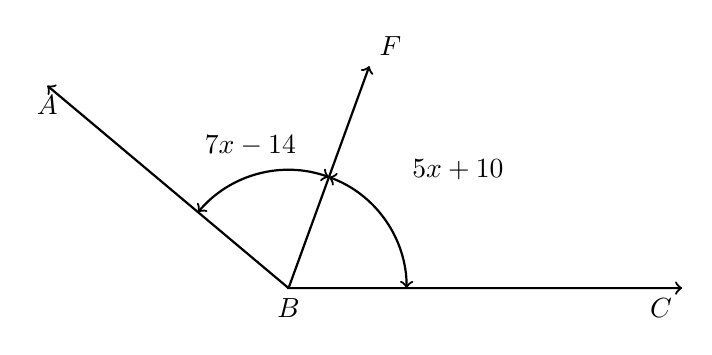
\begin{tikzpicture}[scale=1]
        \draw [<->, thick]
          (0:5) coordinate (a) node[below left] {$C$}
          -- (0,0) coordinate (b) node[below] {$B$}
          -- (70:3) coordinate (c) node[above right] {$F$}
          pic["$5x+10$", <->, draw=black, angle eccentricity=1.75, angle radius=1.5cm]
          {angle=a--b--c};
          \draw [<-, thick]
          (140:4) coordinate (d) node[below] {$A$}
          -- (0,0) coordinate (e)
          pic["$7x-14$", <->, draw=black, angle eccentricity=1.25, angle radius=1.5cm]
          {angle=c--e--d};
          %\draw [->, thick] (0,0)--(-180:2) node[below right]{$A$};
          %\draw (0,0)++(-0.3,0)--++(0,0.3)--+(0.3,0);
      \end{tikzpicture}
    \end{flushright}
    %https://graspablemath.com/canvas?load=_af86aa82e217604b


\end{enumerate}
\end{document}